\section{Software Model}
 
\subsection{Determination of Truss Inertia}

A SolidWorks model exists from initial design of the truss.
Using this model and a material specified as brass, a new coordinate system was created on the top surface of the back mounting washer. 
The corresponds to the axis of rotation for the truss when mounted on the motor.
Then the selected axis was used to determine the value in the Moment of Inertia using MASSPROP function.

\subsection{Controller Design}

The PID controller available in the ACSYS software was used to simulate the system. 
An overall block diagram may be seen in Figure \ref{fig:acsys}.
The built in simulink PID controller is used in the model.
A block diagram for the motor subsystem model is shown in Figure \ref{fig:acsys2}
It should be noted that the correct values for voltage saturation and current saturation were used based on the motor datasheet.

\begin{figure}[ht]
    \centering
    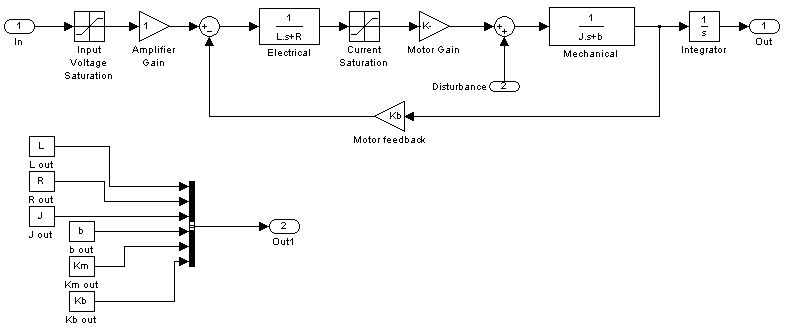
\includegraphics[width=.95\textwidth]{images/acsys2.PNG}
    \caption{Motor Model}
    \label{fig:acsys2}
\end{figure}

\subsection{Simulation}

MATLAB and simulink were used to simulate the motor model and PID controller.
Models available in the ACSYS software package were used.

\subsection{Amplifier Compensation}

The amplifier compensation block diagram may be found in Figure \ref{fig:swpwm}.
It assumes a sampling time of 0.001 seconds.



